\chapter{Background and Related Work}
\label{chap:back}

In this second chapter, we establish the theoretical foundation for our work, covering key concepts in signal processing, anomaly detection, and \acrshort{ai}. We explore relevant data processing techniques and examine previous research on anomaly detection and autoencoders, with a particular focus on methods applicable to \acrshort{das} data.

\section{Digital Signal Processing}

The field of \acrfull{dsp} has been researched since the dawn of time. Signals are all around us, and we do have the means to gather and store the data, but how do we process it more efficiently to be able to analyze and interpret the data in a fast and efficient manner.

When working with \acrshort{das} data in particular, we want to filter the data to remove distortion, and get cleaner outputs to work with. A common way to remove signals outside of a range are called High-pass filters and Low-pass filters. 

A high-pass filter is a function that only allows frequencies above a certain threshold to be accepted, while a low-pass filter only accepts frequencies lower than a threshold $T$. A band-pass filter on the other hand, only allows frequencies within a certain range to be accepted.

\begin{figure}[h]
\centering
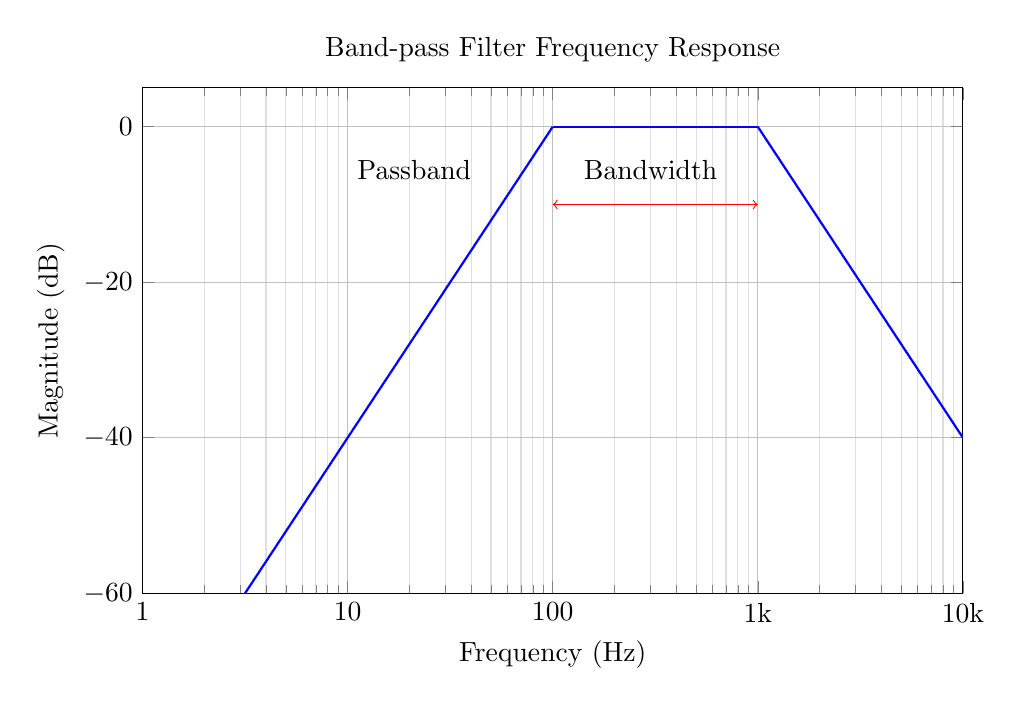
\begin{tikzpicture}
\begin{axis}[
    width=12cm,
    height=8cm,
    xlabel={Frequency (Hz)},
    ylabel={Magnitude (dB)},
    xmode=log,
    xmin=1, xmax=10000,
    ymin=-60, ymax=5,
    xtick={1,10,100,1000,10000},
    xticklabels={1,10,100,1k,10k},
    ytick={-60,-40,-20,0},
    grid=both,
    minor grid style={gray!25},
    major grid style={gray!50},
    title={Band-pass Filter Frequency Response},
]

% Low-frequency rolloff
\addplot[domain=1:100,samples=100,blue,thick] {-40*log10(100/x)};

% Passband
\addplot[domain=100:1000,samples=100,blue,thick] {0};

% High-frequency rolloff
\addplot[domain=1000:10000,samples=100,blue,thick] {-40*log10(x/1000)};

% Annotations
\node[anchor=north west] at (axis cs:10,-3) {Passband};
\draw[<->,red] (axis cs:100,-10) -- (axis cs:1000,-10);
\node[anchor=south] at (axis cs:300,-8) {Bandwidth};

\end{axis}
\end{tikzpicture}
\caption{Ideal Bandpass Filter Response}
\end{figure}


\subsection{Tukey Window}
\label{dsp:tukey}

Window functions are function often used in \acrshort{dsp} and are zero-valued outside of an interval. The Tukey window, also known as the \textit{cosine-tapered window} is one of the more popular window methods, and its mathematical function is described as such: 

\[
    w(x)= 
\begin{cases}
    \frac{1 + \cos{2 \pi \alpha (x + \frac{1-\alpha}{2})}}{2}, & \text{if } x \leq \frac{1-\alpha}{2}\\
    1,              & \text{if } \frac{\alpha}{2} < x \leq \frac{\alpha}{2}\\
    \frac{1 + \cos{2 \pi \alpha (x - \frac{1-\alpha}{2})}}{2}, & \text{if } x > \frac{1-\alpha}{2}
\end{cases}
\]

This window becomes a rectangle when $\alpha = 0$.


\subsection{Resampling}

Also known as sampling-frequency conversion, resampling is the act of modifying the sampling rate of a discrete signal to obtain a new discrete representation of this data. For signal data, lots of samples are usually recorded, but the amount needed to perform calculations or observe patterns does not require this much data. Thus, one can downsample the data to decrease memory usage for storage, as well as time for processing this data. \\


\subsection{Butterworth}

TBI.
\section{Anomaly Detection}
\label{back:anomdet}

\textit{Anomaly detection} is about identifying observations that can be deemed inconsistent with the rest of the dataset \cite{anomaly}. These anomalies can also be referred as outliers, surprises, exceptions, depending on domain. Anomaly detection can be used on all kinds of data, ranging from images to time-series data. There are 3 main types of anomalies, and those are \textit{point anomalies}, \textit{contextual anomalies} and \textit{collective anomalies}.

\begin{figure}[!h]
    \centering
    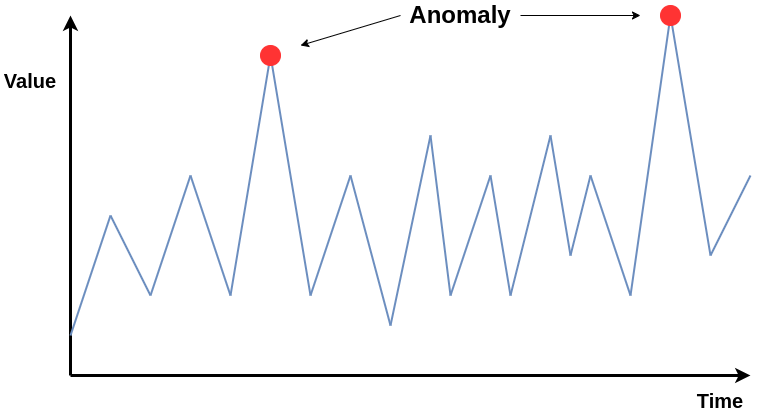
\includegraphics[scale=0.4]{figures/anolay_line.png}
    \caption{Example of anomalies in a time series}
    \label{fig:anomaly_example}
\end{figure}

While point anomalies target single instances that differ from the rest of the dataset, collective anomalies targets groups of instances that together form an anomaly. Contextual ones, as in the word, require context to determine whether or not an anomaly has been detected, and is typically found in time-series data.

Anomaly detection can be performed in a lot of different ways. From common machine learning tasks such as K-means clustering \cite{7507933}, \Gls{svm} \cite{10.1007/978-3-540-28647-9_97}





Given a matrix $a$ of data:

\[
A = \begin{bmatrix}
a_{11} & a_{12} & \cdots & a_{1n} \\
a_{21} & a_{22} & \cdots & a_{2n} \\
\vdots & \vdots & \ddots & \vdots \\
a_{m1} & a_{m2} & \cdots & a_{mn}
\end{bmatrix}
\]

We are interested in finding a region $a_{ij} to a_{kl}$ where $i < k \And j < l$ st. the values within these regions falls outside of the general range


For \acrshort{das} data specifically, anomaly detection can be used for detecting clusters of signals that don't correspond to the predisposed target feature. Registering these outlier signals and receiving real time information about these could prove vital in some cases,  and in best case scenario save lives. 

Dealing with sensitive data 

\subsection{Time series based anomaly detection}

Time series in one dimension is often a great candidate for anomaly detection. Stock market prediction, climate changes and several other series can be used to train networks to recognize point wise anomalies. Layers such as LSTM, RNN and GRU are constructed to store and retrieve information at a later time, thus introducing a memory mechanism. 

\subsection{Image based anomaly detection}

Anomaly detection can also be applied to images. Given a dataset of images with sheep, a image based anomaly detection model would be able to recognize any drastic changes between images. Without the temporal aspect of these problems, convolutional or linear layers are more often used. 

\begin{figure}[!h]
    \centering
    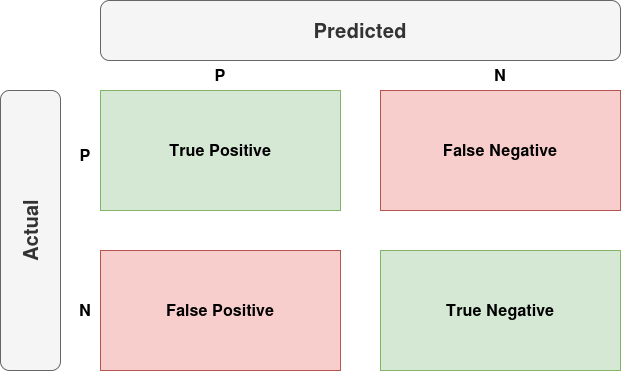
\includegraphics[width=0.5\linewidth]{figures/confmat.png}
    \caption{Caption}
    \label{fig:confmat}
\end{figure}

\section{Unsupervised Learning}

The major bottleneck of all kinds of machine learning tecniques is data. The more diverse and varied a .

When it comes to \acrshort{ai} and \acrshort{ml} we usually differentiate between tree major types, those being supervised, unsupervised and semi-supervised learning (or self-supervised learning). They differ in the roles that can occur.


\subsection{Linear Layers}

Fully Connected Layer, Dense Layer or Linear Layers  are types of an operation used in several deep learning models. This layer take an input vector and maps it to an output of learnable parameters. The resulting parameters are thus a weight matrix $W$ and a bias vector $b$. It is defined as follows:

\begin{align}
    Y &= XW + b
\end{align}

where:
\begin{align*}
    X & \text{ - input vector [$n x m$] where $m$ is the amount of input features and $n$ is the batch size} \\
    W & \text{ - weight matrix [$m x p$] where $p$ is the amount of output features} \\
    b & \text{ - bias vector of size $p$} \\
    Y & \text{ - output vector [$n x p$]} \\
\end{align*}

Furthermore, an activation function such as \gls{relu} \ref{eq:relu} is applied to the output to achieve nonlinearity.
Lets denote this function as $f$, we now get the following equation.

\begin{equation}
    Z = f(Y) = f(XW+b)
\end{equation}

Linear layers have several advantages, such as computational efficiency, flexibility as well as intrerprebility, where the weight and bias vectors can be interpreted as learned parameters. They also serve as building blocks for other components, such as \acrshort{rnn}s, \acrshort{lstm}s or even attention blocks. \\ 

They are however prone to overfitting and linearity, due to their inherent linearity. They can become quite limited when trying to extract more complex features, thus reducing some of the discriminative power.

\subsection{Parallelism within \acrlong{ml}}

With rapid evolving deep learning architectures, the importance of scalable model training and networks grows larger each year. It is even estimated that these networks grow 1,5x each year \cite{9499913}, making parallelization a vital topic when it comes to \acrlong{ml} to accommodate ever increasing memory needs. Several different hardware accelerators have been created to best accommodate these needs, the most apparent of these are \acrshort{gpu}s. NVIDIA have for several years dominated this market, and their hardware is becoming faster and increasing in memory. \\

By workers, we mainly refer to \acrshort{gpu}s, but this could also be processors or other types of hardware accelerators such as TPUs.


\subsubsection{Model Parallelism}

Deep learning models need to store a lot of data. Weights and biases tend to take up a lot of memory, thus requiring the need of splitting up a model across several workers. As an example, given a model $M$ of 50 layers, we can split this model in 2 parts by having a worker $A$ manage the first 25 layers, and worker $B$ manage the latter half.

The overhead of transferring data across these workers can become a bottleneck, so this should only be utilized when absolutely necessary.

\subsubsection{Data Parallelism}

Data parallelism refers to partitioning data across multiple workers.  Given a large set of data, we can split these data across the workers and store a copy of the model on each worker, calculate gradients across them all and update the trainable parameters for the model. An example of this would be to split a batch of size $b$ across $n$ workers, calculate the gradients and update the model. Before updating the parameters of the model, an average across all parameters is calculated, and each of the copies of the model is updated before continuing.

\subsubsection{Hybrid Parallelism}

This kind of parallelization is a combination of the two previously mentioned techniques. By first splitting a model across several workers, data is subsequently split across multiple workers. 
\subsection{Autoencoder}

The autoencoder is a type of network used to learn efficient encodings of unlabeled data. 

Autoencoders are split into two parts. The encoder $E_\phi$ and the decoder $D_\theta$. The relationship between these can be articulated as such: 

\begin{equation}
E_\phi: X \rightarrow Z 
\end{equation}

\begin{equation}
D_\theta: Z \rightarrow X
\end{equation}

The optima for any kind of autoencoder becomes that of lossless encoding, which can further be described as such:

\begin{equation}
    X = D_\theta(E_\phi(X))
\end{equation}

When a auto encoder is trained to max effiency, we can in some cases remove the decoder part. Since the goal in the beginning was to map data to a lower-dimensional latent space, which has been increased. If ones goal is feature extraction, the decoder is not needed any more. Additionally, by removing the decoder, the overall complexity and size of the model $M$ decreases.


Typical usecases for autoencoders are signal analysis, anomaly detection, reconstructing images and so on. 
One of the more well known usages for autoencoders

\subsubsection{Variational Autoencoder (\acrshort{vae})}

Similar to the regular autoencoder, a \acrfull{vae} also aims to map input over to a feature representation. The diffre. Broadly speaking, the difference between a \acrshort{AE} and a \acrshort{VAE} is that a AE maps inpot to points, where as VAEs map over to a distribution in the latent space. Thus, the \acrlong{vae} can be seemed as a generative model.




VAEs can be trained by backpropagation due to something known as the \textit{reparametrization trick}. We need this because since VAEs maps to a stochastic variable, abckpropagation would else not be feasible.

\begin{align*}
\text{Given:} & \quad \text{Encoder LSTM outputs: } h \\
& \quad \text{Mean vector: } \mu \\
& \quad \text{Log variance vector: } \log(\sigma^2) \\
\text{Sample:} & \quad \epsilon \sim \mathcal{N}(0, 1) \\
\text{Reparameterization:} & \quad z = \mu + \sigma \odot \epsilon \\
\text{Decoder Input:} & \quad z \quad \text{(sampled latent vector)} \\
\text{Training Objective:} & \quad \text{Minimize reconstruction error} \\
& \quad \text{and KL divergence between } q(z|x) \text{ and } p(z) \\
\text{Loss Function:} & \quad \mathcal{L} = \text{reconstruction\_loss} + \text{KL\_divergence}
\end{align*}




\subsubsection{LSTM Variational Auto Encoder}

As we've discussed in \ref{ai:lstm} and \ref{ai:rnn}, these types of networks are well suited for . The issues found with \acrshort{rnn}s, such as long term dependencies, are solved with using \acrshort{lstm}s, and also initializing the weights in a more intelligent way. We are not going to make use of transfer learning for our network, thus we solely rely on \acrshort{lstm}s to solve these issues.

Combining the \acrshort{lstm} with an autoencoder approach, we'll be able to create a network well suited for anomaly detection on variable time series data.

\textbf{KEYS TO GETTING A GOOD VARIATIONAL AUTO ENCODER}

\begin{itemize}
    \item Pick the righ size for the latent space
    \item Learning rate scheduler  and hyperparam tuning 
    \item BETA COEFFICIENT
\end{itemize}

An effort has been made into trying to improve autoencoders for anomaly detection \cite{tan2023improving}
\subsubsection{Variational Autoencoder (\acrshort{vae})}
\label{back:vae}

Similar to the regular autoencoder, a \acrfull{vae} also aims to map input over to a feature representation. The diffre. Broadly speaking, the difference between a AE and a \acrshort{vae} is that a AE maps input to points, where as VAEs map over to a distribution in the latent space. The encoder $E$ outputs to vectors. 

Thus, the \acrlong{vae} can be seemed as a generative model.


\begin{figure}[h]
    \centering
    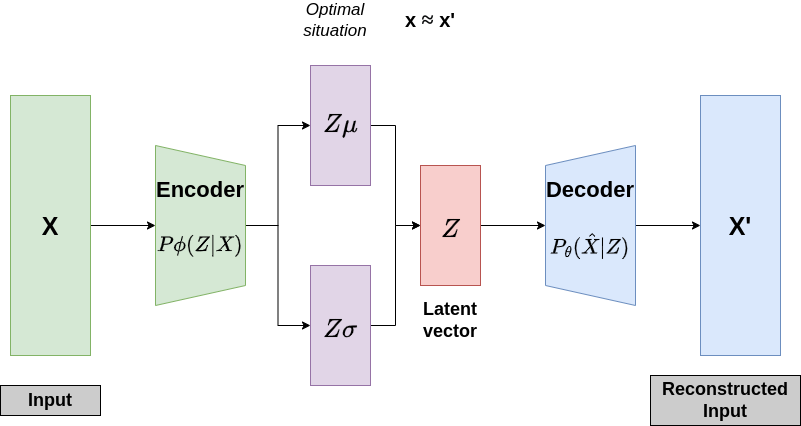
\includegraphics[scale=0.5]{figures/vae.png}
    \caption{Variational Autoencoder Architecture Diagram}
    \label{fig:vaediagram}
\end{figure}


VAEs can be trained by backpropagation due to something known as the \textit{reparametrization trick}. We need this because since VAEs maps to a stochastic variable, abckpropagation would else not be feasible.

\begin{align*}
\text{Given:} & \quad \text{Encoder LSTM outputs: } h \\
& \quad \text{Mean vector: } \mu \\
& \quad \text{Log variance vector: } \log(\sigma^2) \\
\text{Sample:} & \quad \epsilon \sim \mathcal{N}(0, 1) \\
\text{Reparameterization:} & \quad z = \mu + \sigma \odot \epsilon \\
\text{Decoder Input:} & \quad z \quad \text{(sampled latent vector)} \\
\text{Training Objective:} & \quad \text{Minimize reconstruction error} \\
& \quad \text{and KL divergence between } q(z|x) \text{ and } p(z) \\
\text{Loss Function:} & \quad \mathcal{L} = \text{reconstruction\_loss} + \text{KL\_divergence}
\end{align*}


\textbf{KEYS TO GETTING A GOOD VARIATIONAL AUTO ENCODER}

\begin{itemize}
    \item Pick the righ size for the latent space
    \item Learning rate scheduler  and hyperparam tuning 
    \item BETA COEFFICIENT
\end{itemize}

An effort has been made into trying to improve autoencoders for anomaly detection \cite{tan2023improving}

THIS ONE IS HIGHLY RELEVANT AND HAS MANY METRICS \cite{s23021009}
\subsection{Data}
\label{back:data}

\subsubsection{Normalization and Standardization}

Normalization is a technique of which data is transformed from it's original scale, to a more standard scale. These techniques are normally used when the dataset has elements of different ranges. Normalization contribute to faster convergence, and it's why they are as commonly used when preprocessing neural networks. 
The two most common types of normalization are minmax and z score. \\

\textbf{MinMax Normalization}

This algorithm transforms data to a specified range, most often $[0, 1]$ but it can also be $[-1, 1]$ or any other range.
Minmax normalization can be described as follows:

\begin{equation}
   x_{normalized} = \dfrac{x - x_{min}}{x_{max}-x_{min}}
\end{equation}

\textbf{ZScore Standardization}

Contrary to normalization, standardization aims to transform the values to have a mean of 0, and a standard deviation of 1. It also assumes a distribution close to that of a normal one. This method can be expressed as follows. \\ 
\begin{equation}
   x_{standardized} = \dfrac{x - \mu}{\sigma}
\end{equation}

\subsection{Half Precision Training}

Working with large datasets and \acrshort{dnn}s can be rather time- and resource consumptive. To address this, one can cast the datatype from single precision to half precision, along with weights, biases and activations. This will reduce in loss of accuracy and information, but it can drastically lower memory consumption and decrease training time. It is important to note that casting of data occurs with normalization techniques, the order of which operation happens first is quintessential. If the data is casted to half precision before normalization, the normalization will be based on a slightly inaccurate representation of the data, but the computation of the normalized data will be faster. If normalization were to occur first, less detail about the data would be lost, but at the expense of being more computational intensive. \\

\textbf{Mixed precision training}

Mixed precision training, introduced in 2018 \cite{micikevicius2018mixed}, is a technique where the weights, activations and biases of a neural network is stored in single precision, while the data itself stays in it's original format. It allows for reduced memory consumption, while also speeding up operations of deep neural nets. Additionally, the amount of $kwH$ required to train the neural nets would decrease, thus reducing both the cost and the environmental tax by training neural nets. This becomes more important the larger the datasets, models and the sheer amount of GPUS required to train massive workloads. This introduce the concept of loss scaling, where the losses needs to be adjusted based on the weights. \\

\subsection{Datasets}

Loading and processing data before it's trained is a crucial task of constructing any neural networks. In many of the most popular frameworks such as \texttt{Pytorch} and \texttt{TensorFlow}, Datasets and Dataloaders are used to retrieve data from a certain location, transform it to fit the network, and load the data in batches to the model. \\

Datasets are objects that contain information about where to gather the data from, which transformations are to be applied, and functions to gather a single instance of a batch.

\subsection{Dataloaders}

If the datasets contain information about the data and how to retrieve a single instance, the dataloaders job is to create an object that can be iterated over, containing $n$ amount of batches, and transferring these data to the wanted devices. In the case of data parallel multi-gpu training, when the data is loaded, it's \textit{sharded} across the different gpus, in a manner that balances the load of each gpu. Let's say we have a batch  of size $[4, 5, 5]$ and we have two gpus available. The dataloader can split this Tensor in two batches, where each of the gpus get a tensor of size $[2, 5, 5]$. By sharding the data along the first axis, ideally we can half the amount it takes, not taking data transfer time into consideration. 

\begin{figure}[h]
    \centering
    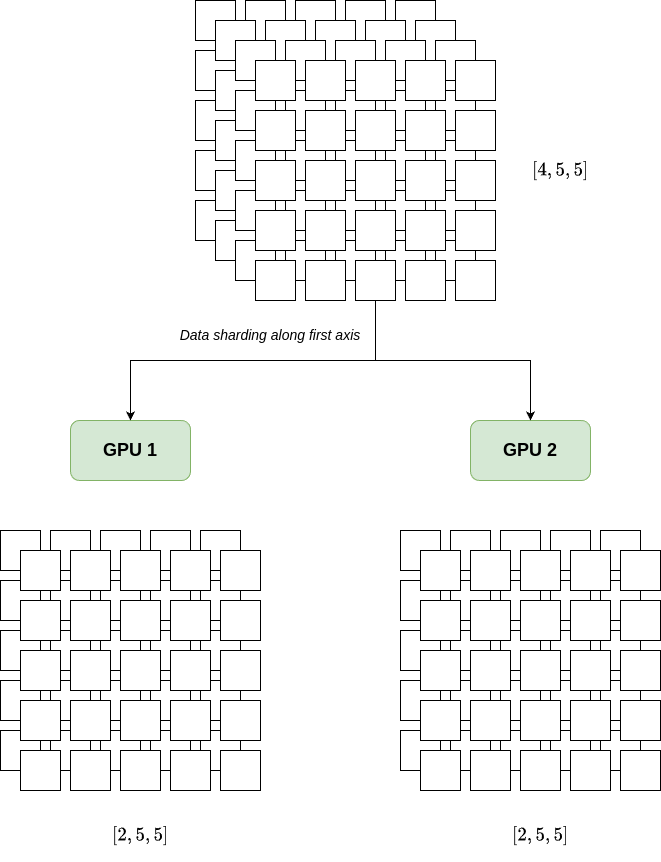
\includegraphics[scale=0.2]{figures/sharding.png}
    \caption{Example of data sharding with 2 gpus, and a original Tensor of size [4,5,5]}
    \label{fig:sharding}
\end{figure}


\textbf{Parallel loading}

When iterating over the dataloader, each element of the batch is retrieved and undergoes transformations. Depending on the batch size and  the size of the data, this procecedure can be very resource-intensice and time-consuming. To mitigate this, we can introduce the concept of parallel batch loading. Instead of gathering and transforming the data sequentially, we instead introduce several workers to be able to do this process in parallel. 

\lstset{style=pstyle}
\lstinputlisting[language=Python]{code/parallel_batch_load.py}
\section{Related Work}
\label{relwork:anomaly}


\subsection{\acrshort{das} file loading and processing}

One of the file formats used for storing \acrshort{das} data is \acrshort{hdf5}. Many of the implemented libraries for \acrshort{hdf5} files now allow for parallel loading of these files. Biddiscombe (et. al 2012) replaced the IO layer within a \acrshort{hdf5} library ''to allow for parallel loading between simulation and analysis'' \cite{biddiscombe2012parallel}. In later years, \texttt{HDF5.jl}, the HDF5 library in Julia, allows for parallel loading of files, utilizing the message-passing interface (MPI). This can potentially reduce \acrshort{das} file loading times. \\ 

An important aspect of \acrshort{das} processing revolves around frequency analysis, denoising, and other types of filtering. 2D \acrfull{fft}s within 2D linear band pass filtering, and one-dimensional adaptive filtering using \acrfull{fir} filters have all been studied and \cite{daspreproc}. In our preliminary studies, we conducted a performance comparison between Julia and Python for computing 2D Fast Fourier Transforms (FFTs) on \acrshort{das} data using \acrshort{gpu}s. Our results demonstrated that Julia significantly outperformed Python in this specific operation \cite{projthesis}. \\

Public \acrshort{das} datasets are often scarce and hard to find. PubDAS \cite{spica2023pubdas} is a public distribution of several \acrshort{das} datasets worldwide, stored in multiple file formats. Many of these datasets contain scripts containing preprocessing algorithms or visualization code. These techniques are sequential, preprocessing file by file and possibly removing erroneous files. These scripts are mainly single-file Python or MatLab scripts. \\ 

One key aspect of \acrshort{ann}s is the necessity of larger train datasets. Data augmentation techniques such as cropping, resizing, or color grading can increase the available datasets for more vision-based tasks. Another way to increase the total amount of train data is by leveraging \acrshort{gan}s. After training a \acrshort{gan} model, the generator can produce data similar to already collected data. This has yielded great results on \acrshort{das} data \cite{Shiloh:19}, and can be a great way to provide more train data, which in turn can help models detect anomalies more accurately by being trained on a wider variety of data. \\

\subsection{Anomaly detection algorithms for \acrshort{das} data analysis}

The most commonly used algorithms regarding machine learning have traditionally been centered around Kmeans clustering, K nearest neighbors, and  Support Vector machines \cite{10.14778/3538598.3538602, 10.1145/3444690}. These have proven to be efficient, especially when dealing with unlabeled data. These clustering techniques are good at outlining groups grouping them, and finding outliers while dealing with them. One article found k means to be a great choice when dealing with traffic analysis and detection \cite{7507933}. Others have looked at svms as another solid option when dealing with anomaly detection \cite{10.1007/978-3-540-28647-9_97}. Omar (et al 2013) \cite{omar2013machine} looked in general at machine learning techniques such as SVMs, k means, decision trees and bayesian networks, and found that supervised ones generally outperforms their unsupervised counterparts when the types of anomalies where known beforehand, but struggle with novel anomalies. \\ 

Alongside well-known clustering techniques such as k means and knn, \acrfull{dbscan}, first published in 1996 \cite{10.5555/3001460.3001507} is a well-known clustering technique suited for outlier detection in multidimensional datasets. It's still being researched and improved as of this date for multivariate time series \cite{waltz2024time}, and has numerous implementations in different frameworks and languages.  


%%%%%%%%%%%%%%%%%%%%%%%%%%%%
%% AE DAS $$$$$ 
%%%%%%%%%%%%%%%%%%%%%%%%%%%%%%%%%%%%%%%%%%%%
An effort has been made into trying to improve autoencoders for anomaly detection \cite{tan2023improving}

Vae for time series \cite{desai2021timevae}


Ball2017 - dl in remote sensing

apSensingo2019railwaydas - powerpoint
s21196627 - dnn microseismic , das
sensors - mdpi ???

In general, autoencoders with linear, convolutional, or recurrent layers, clustering algorithms, and more traditional \acrshort{ml} methods have seen many use-cases within \acrshort{das} research. However, in later years with the later additions of both attention layers, or even \acrshort{gan}s \cite{goodfellow2014generative, goodfellow2016nips}, more novel approaches are being researched. By introducing channel attention and spatial attention to \acrshort{cnn}, one article \cite{eage:/content/journals/10.1111/1365-2478.13355} finds good results for denoising \acrshort{das} signals. 


Label-free autoencoder-based anomaly detection on \acrshort{das} data has been conducted as late as in 2023 \cite{xie2023label}. A combination of a convolutional autoencoder trained on normal-range \acrshort{das} data and a clustering algorithm to locate the feature center was found to beat state-of-the-art supervised networks. Another interesting aspect of this research is the emphasis on model size, creating a sufficient \acrshort{cae} model with only \qty{1.34}{\si{\kilo}} parameters. This research, in particular, has led the ground for our research and the creation of a program for training and comparing several types of autoencoders. \\





\subsection{Other Models}

Zhu (et al. 2023) use ''a pre-trained PhaseNet to generate noisy labels of P/S arrivals in \acrshort{das} data'' and ''applied the GaMMa method to refine noisy labels and build training datasets'' \cite{zhu2023seismic}. A \acrshort{dl} model was then made to detect earthquakes. \\


\acrshort{gan} is another type of generative nn, first proposed by Iain Goodfellow around 2016 \cite{goodfellow2016nips}. These networks have been utilized in models for specifically designed for anomaly detection. A \acrshort{lstm} \acrshort{vae} \acrshort{gan} model was built to detect anomalies within time series \cite{s20133738}. A modification of \acrshort{lstm} \acrshort{gan}, with the inclusion of the attention mechanism \cite{vaswani2017attention}, was built for time-series anomaly detection \cite{bashar2023algan}.ALGAN-DA?
AEGAN-AD \cite{jiang2023unsupervised} uses a \acrshort{gan} based approach to detect anomalies within audio.

Researchers at NTNU constructed a \acrshort{lstm} \acrshort{vae} model for fault detection on a multi-sensor system for maritime systems \cite{9514856} with good success. Deep \acrshort{lstm}-based autoencoders have also been found to be able to detect anomalies within multivariate time-series forecasting problems \cite{alaaDeepLstm2019}.

One issue of concern is online long-distance distributed monitoring applications. By using a combination of a ResNET with a convolutional block attention module (CBAM), one paper is able to achieve real-time inference time cost as low as 3.3ms per sample \cite{photonics9100677}, while still averaging a high accuracy, even for multi-scenario scenes. 


% Huang (et al. 2021) \cite{huang2021esad} semisupervised learning  kl


Anomaly detection, sometimes referred to as outlier detection, is highly relevant within \acrshort{das} research. In 2017, several classical \acrshort{ml} techniques such as Gaussian Mixture Model (GMM), Hidden Markov Model (HMM), Naive Bayes (NB), and Restricted Boltzmann Machine (RBM) were compared to discriminative models, including \acrshort{ann}s \cite{app7080841}. Variations of isolation forests are shown to be able to perform fault detection for mining conveyors\cite{WIJAYA2022110330}. \\

As previously mentioned in chapter \ref{chap:introduction}, label-free anomaly detection has the advantage of requiring a lot less manual labor and can be adapted to multiple datasets. A model that requires only normal-state data, utilizing both autoencoders and the K-means clustering technique, has yielded great results, even beating supervised methods \cite{s23084094}. \\ 

a, \cite{10.14778/3538598.3538602} \cite{10.1145/3444690}.

All this research shows how processing and anomaly detection on \acrshort{das} data is highly relevant. However, most of them do not necessarily concern themselves with available computational power, overall memory consumption, or how to optimize these algorithms for real-time environments, where accuracy, fault tolerance, and inference speed are of utmost importance.



THIS ONE IS HIGHLY RELEVANT AND HAS MANY METRICS \cite{s23021009}
